
To capture gender segregation in the nature of work performed, I construct a \textit{task-based Dissimilarity Index}, denoted $D_{\text{task}}$. This measure extends the standard D index (typically applied to occupational or industry categories) to account for gender differences in task use across occupations.

Each respondent in the SES dataset reports the importance of 11 skill types in their job, using a scale from 0 to 4:

\begin{itemize}
    \item 0 = Does not apply in job
    \item 1 = Not very important
    \item 2 = Fairly important
    \item 3 = Very important
    \item 4 = Essential
\end{itemize}

To simplify the construction of a task use indicator, I convert each continuous skill score into a binary indicator, where a skill is considered used if its value exceeds 2.5:

\[
\text{TaskUsed}_{i,s} =
\begin{cases}
1 & \text{if } \text{Skill}_{i,s} > 2.5 \\
0 & \text{otherwise}
\end{cases}
\]

for individual $i$ and skill $s$. I then compute, for each occupation $j$ and skill $s$, the weighted share of men and women who report using the skill, using grossing weights $w_i = \text{gwtall}$. Let:

\begin{itemize}
    \item $M_{j,s}$ = weighted number of men in occupation $j$ using skill $s$
    \item $F_{j,s}$ = weighted number of women in occupation $j$ using skill $s$
    \item $T^M_j$, $T^F_j$ = total weighted men and women in occupation $j$
\end{itemize}

Then the task-level gender difference is:

\[
d_{j,s} = \left| \frac{M_{j,s}}{T^M_j} - \frac{F_{j,s}}{T^F_j} \right|
\]

If either gender is absent from occupation $j$, I assign $d_{j,s} = 1$, reflecting complete segregation.

I then compute the mean difference across all skills within occupation $j$:

\[
D_j = \frac{1}{S} \sum_{s=1}^{S} d_{j,s}
\]

where $S = 11$ is the number of skills. This yields an occupation-level segregation score $D_j \in [0, 1]$.

Finally, I compute the aggregate index in two forms:

\textbf{Unweighted average:}
\[
D_{\text{task}}^{\text{unweighted}} = \frac{1}{J} \sum_{j=1}^{J} D_j
\]

\textbf{Weighted average:}
\[
D_{\text{task}}^{\text{weighted}} = \sum_{j=1}^{J} \left( \frac{W_j}{\sum_{j=1}^{J} W_j} \right) D_j
\]

This index reflects the extent to which men and women perform different tasks across occupations, even when working in similar jobs or industries. 
It captures a dimension of gender segregation that is not visible through occupation or industry codes alone.

Figure X displays trends in gender task segregation across UK occupations from 1997 to 2017, measured using a 
modified version of the Duncan Dissimilarity Index. The figure distinguishes between an unweighted version of 
the index, which gives equal weight to each occupation, and a weighted version that adjusts for the employment 
size of occupations to reflect aggregate worker experience.

The unweighted index reveals persistently moderate levels of task segregation, with values ranging from 52.7% 
in 1997 to 46.5\% in 2017. Although there is an overall decline across the two decades, the pattern is non-linear, 
with a noticeable dip in 2006 followed by a rebound in 2012. This suggests that the degree of task differentiation 
between men and women within occupations remains substantial and relatively stable when each occupation is treated 
equally, regardless of size.

By contrast, the weighted index—which accounts for the number of individuals employed in each occupation—shows a 
consistently lower level of task segregation, ranging from 36.9\% in 2006 to 34.8\% in 2012, and ending at 32.2% in 
2017. This indicates that the average worker in the labour market experiences significantly lower task segregation 
than the unweighted average suggests, implying that larger occupations tend to exhibit more gender-integrated task 
profiles.

The divergence between the weighted and unweighted trends underscores the importance of accounting for employment 
size when assessing the extent of gender segregation. While smaller occupations may exhibit higher levels of gendered 
task differentiation, they employ fewer individuals and therefore contribute less to aggregate patterns. The weighted 
index suggests a modest downward trend in task segregation over time, albeit from already relatively low levels. 
Together, these findings point to a persistent but gradually declining pattern of gender-based task differentiation 
within occupations, with significant variation across the occupational structure.

\begin{figure}[!t]
    \centering
    \caption{Task Seggregation}
    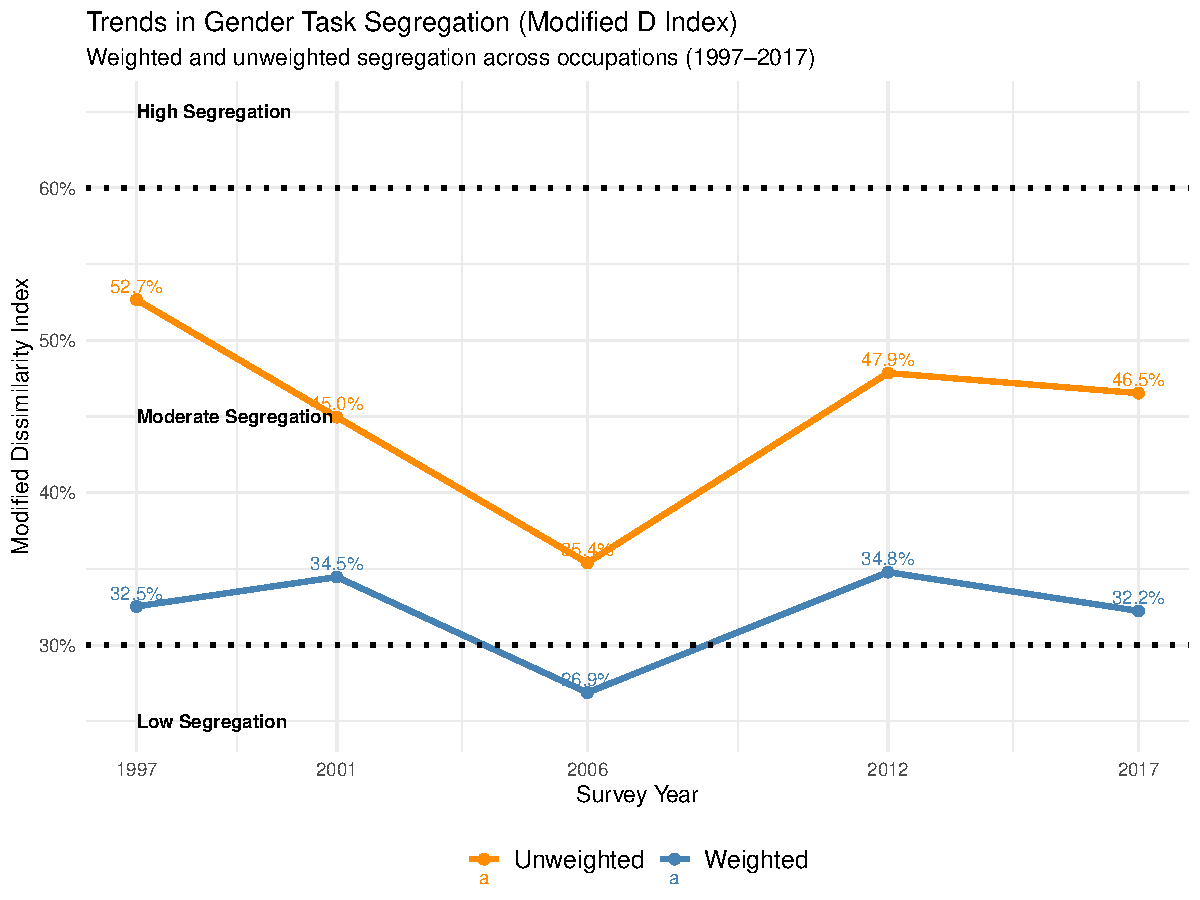
\includegraphics[width=\textwidth]{_graphic/task_segregation.pdf}
    \label{fig:task_segregation}
    \vspace{-3em}
    \justify\singlespacing\scriptsize\textit{Notes}: Notes here.
\end{figure}



\begin{figure}[!t]
    \centering
    \caption{Title}
    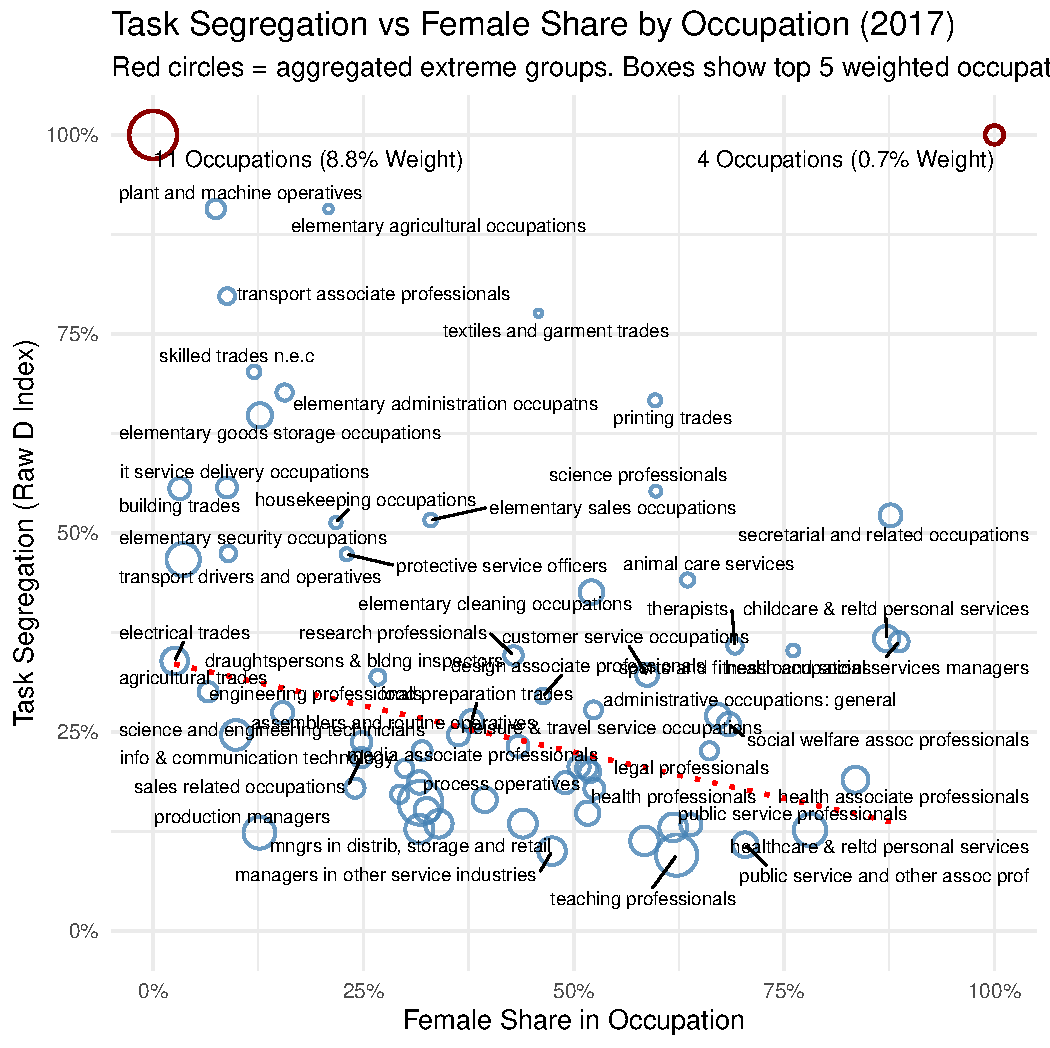
\includegraphics[width=\textwidth]{_graphic/task_b3occ_females_share_nobox.pdf}
    \label{fig:task_b3occ_females_share_nobox}
    \vspace{-3em}
    \justify\singlespacing\scriptsize\textit{Notes}: Notes here.
\end{figure}

The scatter plot illustrates the relationship between task segregation and female occupational share 
in the UK labour market in 2017. Each point represents a 3-digit SOC occupation, with task segregation 
measured by the modified D on the vertical axis and the proportion of women in each occupation 
on the horizontal axis. A negative association emerges: occupations with a higher share of women 
tend to exhibit lower levels of task segregation, suggesting that in more gender-balanced or female-dominated 
roles, men and women are more likely to perform similar tasks. This pattern is captured by the downward-sloping 
trend line, indicating that gender-based task differentiation diminishes as female representation increases.

However, beyond this general trend, a number of occupations lie well above the trend line, indicating 
significantly higher levels of task segregation than would be predicted based on their gender composition 
alone. These outliers are concentrated in both male- and female-dominated fields, revealing that high task 
segregation is not confined to one side of the gender distribution. On the male-dominated side, occupations 
such as plant and machine operatives, transport associate professionals, and skilled trades (not elsewhere classified) 
display relatively high levels of task segregation, even after accounting for their low female share. 
On the female-dominated side, occupations such as textiles and garment trades, printing trades, and science 
professionals also show elevated levels of task segregation despite having moderate to high female representation.

These patterns suggest that in some occupations, the division of tasks between men and women is especially 
pronounced. In these cases, gendered role 
expectations or organizational structures may contribute to sharp internal task differentiation. 
Such deviations from the average pattern highlight the importance of examining within-occupation task 
segregation directly, rather than relying solely on measures of occupational gender composition, in order 
to uncover the mechanisms through which gendered labour market inequalities are maintained.